\documentclass[ngerman]{gdb-aufgabenblatt}
\RequirePackage[utf8]{inputenc}
\renewcommand{\Aufgabenblatt}{3}
\renewcommand{\Ausgabedatum}{Mi. 13.11.2013}
\renewcommand{\Abgabedatum}{Do. 28.11.2013}
\renewcommand{\Gruppe}{Tim Dittrich, Sebastian Lindemann, Jim Martens}

% define how the sections are rendered
\def\thesection{Aufgabe \arabic{section}:}
\def\thesubsection{\alph{subsection})}
\def\thesubsubsection{(\roman{subsubsection})}

\usetikzlibrary{positioning}
\usetikzlibrary{shadows}

\begin{document}
\section{Relationenalgebra}
	\subsection{} %a
		\[
			\pi_{Obst.Sorte}(Obst \underset{Obst.Entdecker=Person.PNR}{\bowtie}( \sigma_{Vorname='Horst'}(Person)))
		\]
	\subsection{} %b
		\[
			\pi_{Person.Vorname, Person.Nachname}(Person \underset{Person.PNR=Allergie.Person}{\bowtie} (\sigma_{Symptom='Halskratzen'}(Allergie)))
		\]
	\subsection{} %c
		\[
			\pi_{Obst.Sorte, Person.Nachname}((Person \underset{Obst.Entdecker=Person.PNR}{\bowtie} Obst) \underset{Allergie.Obst=Obst.ONR}{\bowtie} (\sigma_{Symptom='W"urgreiz'}(Allergie)))
		\]
		
\section{SQL - Schemadefinition}
	\subsection{} %a
		\begin{verbatim}
		    CREATE TABLE Rennstall (
		        RSID      INT(10)      NOT NULL PRIMARY KEY,
		        Name      VARCHAR(255) NOT NULL UNIQUE KEY,
		        Teamchef  VARCHAR(255) DEFAULT NULL,
		        Budget    INT(3)       NOT NULL CHECK(Budget>=0 AND Budget <= 500)
		    );
		    
		    CREATE TABLE Rennfahrer (
		        RID       INT(10)      NOT NULL PRIMARY KEY,
		        Rennstall INT(10)      NOT NULL,
		        Vorname   VARCHAR(255) NOT NULL,
		        Nachname  VARCHAR(255) NOT NULL,
		        Geburt    DATE         NOT NULL,
		        Wohnort   VARCHAR(255) DEFAULT NULL,
		        CONSTRAINT fk_rennstall FOREIGN KEY (Rennstall) REFERENCES Rennstall (RSID)
		    );
		    
		    CREATE TABLE Rennort (
		        OID       INT(10)      NOT NULL PRIMARY KEY,
		        Name      VARCHAR(255) NOT NULL,
		        Strecke   VARCHAR(255) NOT NULL
		    );
		    
		    CREATE TABLE Platzierung (
		        RID       INT(10)      NOT NULL,
		        OID       INT(10)      NOT NULL,
		        Platz     INT(3)       NOT NULL,
		        CONSTRAINT pk_platzierung PRIMARY KEY (RID, OID)
		    );
		\end{verbatim}
	\subsection{} %b
		Dadurch muss beim Erstellen einer Datenbankabfrage verstärkt darauf geachtet werden, dass nach jeder einzelnen Anweisung die Integrität eingehalten wird. Demnach wird eine feste Reihenfolge vorgegeben. Zyklische Verweise verhindern damit ein irgendwie geartetes Verändern auch nur eines Bestandteils, wenn durch diese Änderung irgendeine Fremdschlüsselbedingung verletzt ist.
		
		Der Fremdschlüssel von Rennstall zu Rennfahrer könnte erst nach der Anlegung der Tabelle Rennfahrer erstellt werden.
		
		Außerdem könnten dadurch weder Rennställe noch Rennfahrer gelöscht werden. Wenn ein Rennfahrer gelöscht werden soll und er ein Star eines Rennstalles ist, dann wird die Operation sofort abgebrochen. Umgekehrt kann kein Stall gelöscht werden, da zumindest der Star des Rennstalles selber auf den Rennstall referenziert, wodurch auch solche eine Operation abgebrochen würde.
	\subsection{} %c
	\begin{verbatim}
	    INSERT INTO Rennstall
	                  (RSID, Name, Teamchef, Budget)
	           VALUES (2, 'Red Bull', 'Christian Horner', 370),
	                  (5, 'Ferrari', 'Stefano Domenicali', 350),
	                  (31, 'McLaren', 'Martin Whitmarsh', 220),
	                  (34, 'Lotus F1', 'Eric Boullier', 100);
	    
	    INSERT INTO Rennfahrer
	                  (RID, Rennstall, Vorname, Nachname, Geburt, Wohnort)
	           VALUES (4, 2, 'Sebastian', 'Vettel', 19870703, 'Kemmental (Schweiz)'),
	                  (6, 5, 'Fernando', 'Alonso', 19810729, 'Lugano (Schweiz)'),
	                  (8, 2, 'Marc', 'Webber', 19760827, 'Aston Clinton (UK)'),
	                  (9, 31, 'Lewis', 'Hamilton', 19850107, 'Genf (Schweiz)'),
	                  (20, 31, 'Jenson', 'Button', 19800119, 'Monte Carlo (Monaco)'),
	                  (21, 5, 'Felipe', 'Massa', 19820425, 'São Paulo (Brasilien)'),
	                  (44, 34, 'Kimi', 'Räikkönen', 19791017, 'Espoo (Finnland)');
	                  
	    INSERT INTO Rennort
	                  (OID, Name, Strecke)
	           VALUES (4, 'Australien GP', 'Albert Park Circuit'),
	                  (15, 'Malaysia GP', 'Sepang International Circuit'),
	                  (21, 'China GP', 'Shanghai International Circuit');
	                  
	    INSERT INTO Platzierung
	                  (RID, OID, Platz)
	           VALUES (8, 4, 6),
	                  (4, 15, 1),
	                  (20, 15, 17),
	                  (4, 4, 3),
	                  (6, 4, 2),
	                  (8, 15, 2),
	                  (6, 21, 1),
	                  (9, 4, 5),
	                  (21, 15, 5),
	                  (20, 4, 9),
	                  (21, 4, 4); 
	\end{verbatim}
	\subsection{} %d
		
		\begin{itemize}
			\item \begin{verbatim}
			    DELETE FROM Rennfahrer
			    WHERE       Vorname LIKE 'F%';
			\end{verbatim}	
			\item \begin{verbatim}
			    DROP TABLE Platzierung;
			    DROP TABLE Rennort;
			    DROP TABLE Rennfahrer;
			    DROP TABLE Rennstall;
			\end{verbatim}
		\end{itemize}

\section{SQL - Anfragen}
	\subsection{} %a
		\begin{verbatim}
		    SELECT DISTINCT obst.Sorte
		    FROM            Person pers,
		                    Allergie aller,
		                    Obst obst
		    WHERE           pers.PNR = aller.Person
		    AND             aller.Obst = obst.ONR
		    AND             pers.Vorname = 'Peter'
		    AND             pers.Nachname = 'Meyer'
		    ORDER BY        obst.Sorte DESC;
		\end{verbatim}
	\subsection{} %b
		\begin{verbatim}
		    SELECT   pers.PNR, pers.Nachname, COUNT(aller.Obst)
		    FROM     Person pers,
		             Allergie aller
		    WHERE    pers.PNR = aller.Person
		    GROUP BY pers.PNR;
		\end{verbatim}
	\subsection{} %c
		\begin{verbatim}
		    SELECT   pers.PNR
		    FROM     Person pers,
		             Obst obst
		    WHERE    pers.PNR = obst.Entdecker
		    GROUP BY pers.PNR
		    HAVING   COUNT(obst.ONR) > 6;
		\end{verbatim}
	\subsection{} %d
		\begin{verbatim}
		    SELECT pers.Vorname, pers.Nachname
		    FROM   Person pers,
		           Person entdecker,
		           Obst obst
		    WHERE  entdecker.PNR = obst.Entdecker
		    AND    pers.Lieblingsobst = obst.ONR
		    AND    entdecker.Vorname = pers.Vorname;
		\end{verbatim}
	\subsection{} %e
		\begin{verbatim}
		    SELECT   pers.PNR, pers.Vorname, pers.Nachname
		    FROM     Person pers
		    WHERE    pers.PNR NOT IN (SELECT obst.Entdecker
		                              FROM   Obst obst);
		\end{verbatim}

\section{Optimierung}
	anfänglicher Operatorbaum:\\
	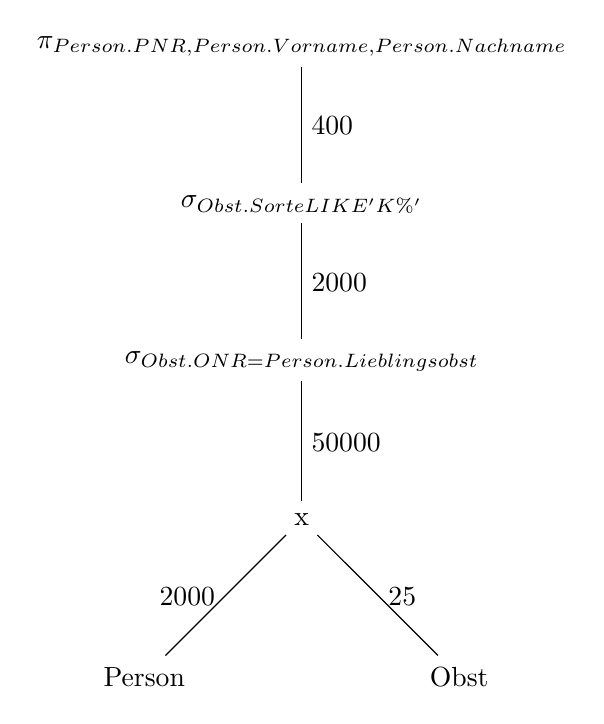
\begin{tikzpicture}[shorten >=1pt,node distance=1.1cm,on grid]
		\node (proj) {$\pi_{Person.PNR, Person.Vorname, Person.Nachname}$};
		\node (sel) [below=2.0 of proj] {$\sigma_{Obst.Sorte\text{ LIKE 'K\%'}}$};
		\node (sel2) [below=2.0 of sel] {$\sigma_{Obst.ONR=Person.Lieblingsobst}$};
		\node (catProd) [below=2.0 of sel2] {x};
		\node (person) [below left=2.0 and 2.0 of catProd] {Person};
		\node (obst) [below right=2.0 and 2.0 of catProd] {Obst};
		\path (proj) edge node [right] {400} (sel)
			  (sel) edge node [right] {2000} (sel2)
		      (sel2) edge node [right] {50000} (catProd)
		      (catProd) edge node [left] {2000} (person)
		      (catProd) edge node [right] {25} (obst);
	\end{tikzpicture}
	
	optimierter Operatorbaum:\\
	\begin{tikzpicture}[shorten >=1pt,node distance=1.1cm,on grid]
		\node (proj) {$\pi_{Person.PNR, Person.Vorname, Person.Nachname}$};
		\node (join) [below=2.0 of proj] {$\underset{Person.Lieblingsobst = Obst.ONR}{\bowtie}$};
		\node (person) [below left=2.0 and 2.0 of join] {Person};
		\node (sel) [below right=2.0 and 2.0 of join] {$\sigma_{Obst.Sorte\text{ LIKE 'K\%'}}$};
		\node (obst) [below=of sel] {Obst};
		\path (proj) edge node [right] {400} (join)
		      (join) edge node [left] {2000} (person)
		      (join) edge node [right] {5} (sel)
		      (sel) edge node [right] {25} (obst);
	\end{tikzpicture}
	
	Der zweite Operatorbaum ist klar performanter, da die Selektion der Obstsorte bereits vor dem Join stattfindet und das kartesische Produkt und die zweite Selektion zu einem Join verbunden wurde.
\end{document}